\section{Division by auto-power spectrum}
\label{appendix:W_filtering}
In section \ref{sec:corr_based_approach}, the following filter is defined.
\begin{equation*}
    W(q^{-1}) = \frac{F(q^{-1})(1-M(q^{-1}))}{S_{UU}(q^{-1})}
\end{equation*}
with $S_{UU}(q^{-1})$ being a parametric representation of the auto-power spectrum of $u(n)$.

If $u(n)$ is DT filtered white noise $u(n) = S_u(q^{-1}) e_u(n)$ and a parametric representation of $S_u(q^{-1})$ is known, then the auto-power spectrum of $u(n)$ becomes
\begin{equation*}
    S_{UU}(q^{-1}) = S_u(q^{-1}) S_u(q)
\end{equation*}
The zeros of $S_u(q^{-1})$ and $S_u(q)$ have an inverse relationship. If $a$ is a zero of $S_u(q^{-1})$, then $a^{-1}$ is a zero of $S_u(q)$. These zeros then become poles of $W(q^{-1})$. Thus, if $S_u(q^{-1})$ contains zeros that are not on the unit circle, the filter $W(q^{-1})$ will be unstable. And so, applying the filter in the time domain is in general not possible.

\newpage
\section{DFT of cross-correlation}
\label{appendix:DFT_cross}
The circular cross-correlation of two discrete signals $x$ and $y$ is defined by \cite[eq. (2.22) ]{Wang_crosscorrelation}
\begin{equation}
    R_{xy}(\tau) = \sum_{n = 0}^{N-1} \overline{x(n)} y(\text{mod}(n+\tau,N)) 
    \label{eq:R_xy}
\end{equation}
Taking the DFT of (\ref{eq:R_xy}) gives
\begin{align*}
    S_{XY}(k) &= \frac{1}{N}\sum_{\tau = 0}^{N-1} R_{xy}(\tau) e^{-j2\pi k \tau /N} = \frac{1}{N}\sum_{\tau = 0}^{N-1} \sum_{n = 0}^{N-1} \overline{x(n)} y(\text{mod}(n+\tau,N))  e^{-j2\pi k \tau /N}\\
    &= \frac{1}{N}\sum_{n = 0}^{N-1} \overline{x(n)} \sum_{\tau = 0}^{N-1} y(\text{mod}(n+\tau,N))  e^{-j2\pi k \tau /N} \\
    &= \frac{1}{N}\sum_{n = 0}^{N-1} \overline{x(n)} e^{j2\pi k t/N} \sum_{\tau = 0}^{N-1} y(\text{mod}(n+\tau,N))  e^{-j2\pi k (n+\tau) /N}
\end{align*}
The second sum is actually independent of $n$.
\begin{align*}
    \sum_{\tau = 0}^{N-1} y(\text{mod}(n+\tau,N))  e^{-j2\pi k (n+\tau) /N} &= \sum_{\tau = 0}^{N-t-1} y(n+\tau)  e^{-j2\pi k (n+\tau) /N}\\ & + \sum_{\tau = N-t}^{N-1} y(n+\tau-N)  e^{-j2\pi k (n+\tau) /N} \\
    &= \sum_{\tau = 0}^{N-t-1} y(n+\tau)  e^{-j2\pi k (n+\tau) /N}\\ & + \sum_{\tau = -t}^{-1} y(n+\tau)  e^{-j2\pi k (n+\tau+N) /N} \\
    & = \sum_{\tau = -t}^{N-t-1} y(n+\tau)  e^{-j2\pi k (n+\tau) /N}
\end{align*}
In the last step we used the fact that $e^{-j2\pi k (n+\tau+N) /N} = e^{-j2\pi k (n+\tau) /N}$. Now by doing one last substitution we get
\begin{align*}
    \sum_{\tau = 0}^{N-1} y(\text{mod}(n+\tau,N))  e^{-j2\pi k (n+\tau) /N} = \sum_{\tau = 0}^{N-1} y(\tau) e^{-j2\pi k \tau /N}
\end{align*}
This equation is valid because the sum runs over all the samples $0,\ldots,N-1$. Finally, the DFT of the cross-correlation is
\begin{align*}
    S_{XY}(k) &= \frac{1}{N} \overline{\sum_{n = 0}^{N-1} x(n) e^{-j2\pi k t/N}} \sum_{\tau = 0}^{N-1} y(\tau)  e^{-j2\pi k \tau /N} \\
    \Rightarrow S_{XY}(k) &=  N \overline{X(k)} Y(k)
\end{align*}

\newpage
\section{Unstable systems}
\label{appendix:unstable}
Open loop experiments are not practical on unstable systems. If we want to measure the FRF of an unstable system, it will have to be done in closed loop with a stabilizing controller. As discussed in section \ref{sec:feedback}, the danger here is that process noise on the output will be fed back to the input. Not taking the right precautions will lead to an inconsistent nonparametric estimate of the FRF in some cases.

First, a quick summary of the solution given in \cite{Data-driven_model_reference_control} will be discussed. Then it will be shown that a nonparametric estimate of the FRF is again hidden in the maths.

\subsection{Correlation-based approach}
\paragraph{Model}
The set-up shown in figure \ref{fig:unstable_system} is considered. An unstable system $G(q^{-1})$ is stabilized by a controller $K_s(q^{-1})$ in negative feedback. The reference signal $r(n)$ is entered between the controller and the system. The reference signal is assumed to be periodic. The input to the system is $u(n)$ and the output of the system $y(n)$ is perturbed by process noise $v(n)$. The signal $x(n)$ is the reference signal that would be used in the actual closed loop system. However, to keep the notation similar to \cite{Data-driven_model_reference_control}, $x(n)$ is set to 0. The closed loop TF from $x(n)$ to $y(n)$ is
\begin{equation*}
    M_s(q^{-1}) = \frac{K_s(q^{-1}) G(q^{-1})}{1 + K_s(q^{-1}) G(q^{-1})}
\end{equation*}

\begin{figure}[H]
    \centering
    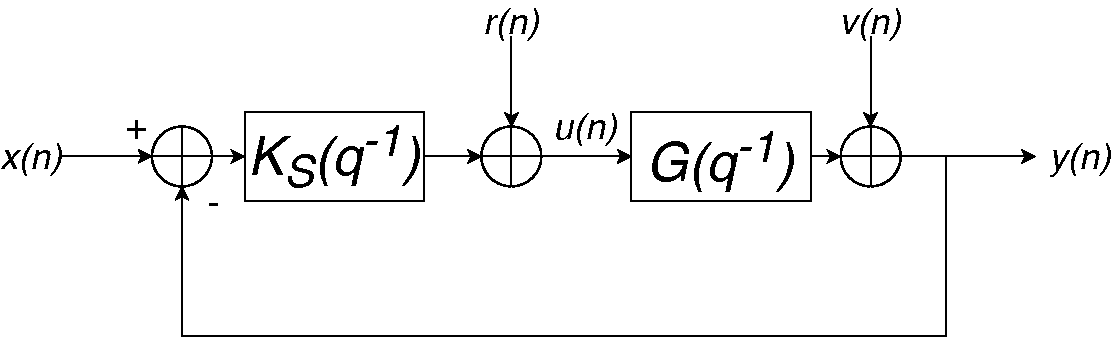
\includegraphics[width = 0.65\textwidth]{figures/unstable_system.pdf}
    \caption{Unstable LTI system with a stabilizing controller in feedback.}
    \label{fig:unstable_system}
\end{figure}

\paragraph{Error signal} The error signal is the same as in section \ref{sec:corr_based_approach}.
\begin{equation*}
    \epsilon(n,\rho) = M u(n) - K(\rho) (1 - M) y(n)
\end{equation*}

\paragraph{Reference filtering}
This time, the reference signal $r(n)$ is filtered instead of the input to the system $u(n)$. The filter $W(q^{-1})$ which is used to obtain $r_W(n)$ is defined differently this time.
\begin{equation}
    W(e^{-j\omega}) = \frac{F(e^{-j\omega}) (1-M(e^{-j\omega}))}{(1-M_s(e^{-j\omega})) S_{RR}(e^{-j\omega})}
    \label{eq:W_unstable_non-practic}
\end{equation}
with $S_{RR}(e^{-j\omega})$ being the auto-power spectrum of the reference signal. It is pointed out in \cite{Data-driven_model_reference_control} that $W(e^{-j\omega})$ cannot be implemented in this way, because $M_s$ is not known as we don't have access to a parametric representation of $G$. This is solved in the following way. First, $u(n)$ is written as a function of $r(n)$ and $v(n)$.
\begin{equation*}
    u(n) = \frac{1}{1+K_s G} r(n) - \frac{K_s}{1+K_s G} v(n)
\end{equation*}
Assuming that there is no noise $v(n) = 0$ and rewriting $1+K_s G$ in terms of $M_s$, gives
\begin{equation*}
    u(n) = (1-M_s) r(n)
\end{equation*}
Hence, there is a relation between the auto-power spectrum of $r(n)$ and the cross-power spectrum between $r(n)$ and $u(n)$.
\begin{equation*}
    S_{RU}(e^{-j\omega}) = (1-M_s(e^{-j\omega})) S_{RR}(e^{-j\omega})
\end{equation*}
And so (\ref{eq:W_unstable_non-practic}) becomes
\begin{equation*}
    W(e^{-j\omega}) = \frac{F(e^{-j\omega}) (1-M(e^{-j\omega}))}{S_{RU}(e^{-j\omega})}
\end{equation*}
$S_{RU}(e^{-j\omega})$ can be estimated from the data and the filter can be applied to $r(n)$ in the FD to obtain $r_W(n)$.

\paragraph{Correlation criterion}
Then, the cross-correlation between $r_W(n)$ and $\epsilon(n,\rho)$ is calculated.
\begin{equation*}
    R_{r_W \epsilon}(\tau,\rho) = \frac{1}{N\!P} \sum_{n=0}^{N\!P-1} r_W(n-\tau) \epsilon(n,\rho)
    % \label{eq:RuWepstau_unstable}
\end{equation*}
with $P$ being the number of periods measured. The cost function can then be calculated by using (\ref{eq:JNl1}).

\subsection{Nonparametric estimate}
The error signal in the FD becomes
\begin{equation*}
    E(kP,\rho) = M(\Omega_k) U(kP) - K(\Omega_k,\rho) (1-M(\Omega_k)) Y(kP)
\end{equation*}
Here, because the reference signal is periodic, the frequencies $\Omega_k$ correspond to the DFT bins $kP$. For the rest of this section, the frequencies $\Omega_k$ will be left out from the equations for clarity.
The filtered reference signal becomes
\begin{equation*}
    R_W(kP) = \frac{F (1-M) R(kP)}{R(kP) \overline{U(kP)}}
\end{equation*}
Then the cross-power spectrum between $\epsilon(n,\rho)$ and $r_W(n)$ is
\begin{align*}
    S_{R_W\!E}(\Omega_k,\rho) &= R_W(kP) \overline{E(kP,\rho)} = F(1-M) \overline{\Big[M \frac{U(kP) \overline{R(kP)}}{U(kP) \overline{R(kP)}} - K(\rho) (1-M) \frac{Y(kP) \overline{R(kP)}}{U(kP) \overline{R(kP)}}\Big]}\\
    &= F(1-M) \overline{[M - K(\rho) (1-M) \hat{G}(\Omega_k) ]}
\end{align*}
with 
\begin{equation}
    \hat{G}(\Omega_k) = \frac{Y(kP) \overline{R(kP)}}{U(kP) \overline{R(kP)}} = \frac{Y(kP)}{U(kP)}
    \label{eq:G=Y(kP)/U(kP)_unstable}
\end{equation}
If $\hat G$ is replaced by the actual system $G$, $S_{R_W\!E}(\Omega_k,\rho)$ is exactly the quantity being integrated over in (\ref{eq:J}). As was discussed in section \ref{sec:corr_based_approach}, (\ref{eq:G=Y(kP)/U(kP)_unstable}) is equivalent to taking the DFT of every period and taking the mean of the spectra over the periods.
\begin{equation*}
    \hat G(\Omega_k) = \frac{\frac{1}{P}\sum_{p=0}^{P-1}  Y^{(p)}(k)}{\frac{1}{P}\sum_{p=0}^{P-1}  U^{(p)}(k)}
\end{equation*}
Note that this estimate is consistent when the excitation is periodic. For arbitrary excitations it is inconsistent. It is interesting to see that the unsimplified fraction in (\ref{eq:G=Y(kP)/U(kP)_unstable}) looks like the indirect method for estimating the FRF (see section \ref{sec:feedback}).
\begin{equation*}
    \hat G(\Omega_k) = \frac{ \frac{1}{P}\sum_{m=0}^P Y^{(m)}(k) \overline{R^{(m)}(k)} } { \frac{1}{P}\sum_{m=0}^P U^{(m)}(k) \overline{R^{(m)}(k)} }
\end{equation*}
This FRF estimate is consistent when using arbitrary excitations.